
%(BEGIN_QUESTION)
% Copyright 2011, Tony R. Kuphaldt, released under the Creative Commons Attribution License (v 1.0)
% This means you may do almost anything with this work of mine, so long as you give me proper credit

A 480 volt AC three-phase electrical system provides power to an induction motor:

$$\includegraphics[width=15.5cm]{i03503x01.eps}$$

Calculate the source's line current, assuming 100\% efficiency for the motor, and a perfect (1.0) power factor.

\vskip 10pt

$I_{line}$ = \underbar{\hskip 50pt} amps

\vskip 50pt

Next, calculate the amount of current through the AC ammeter given a CT ratio of 100:5, and the amount of voltage present at the AC voltmeter given a PT ratio of 150:1.

\vskip 10pt

$I_{meter}$ = \underbar{\hskip 50pt} amps

\vskip 10pt

$V_{meter}$ = \underbar{\hskip 50pt} volts

\underbar{file i03503}
%(END_QUESTION)





%(BEGIN_ANSWER)

{\it 4 points for line current, 3 points for each meter reading.}

\vskip 10pt

$I_{line}$ = \underbar{\bf 13.46} amps

\vskip 10pt

$I_{meter}$ = \underbar{\bf 0.673} amps

\vskip 10pt

$V_{meter}$ = \underbar{\bf 3.2} volts

%(END_ANSWER)





%(BEGIN_NOTES)

{\bf This question is intended for exams only and not worksheets!}.

%(END_NOTES)

